\documentclass[dutch, oneside]{tudelft-report}

\begin{document}
\chapter{Design overview and system design}
Het systeem is opgedeeld in vier blokken:
\begin{itemize}
\item De main controller
\item De DCF controller
\item LCD controller
\item Alarm
\end{itemize}

\noindent In figuur \ref{fig:blokdiagram} is te zien welke ingangs- en uitgangssignalen het systeem in en uit gaan en hoe de blokken elkaar aansturen.

\begin{figure}[h!]
\center
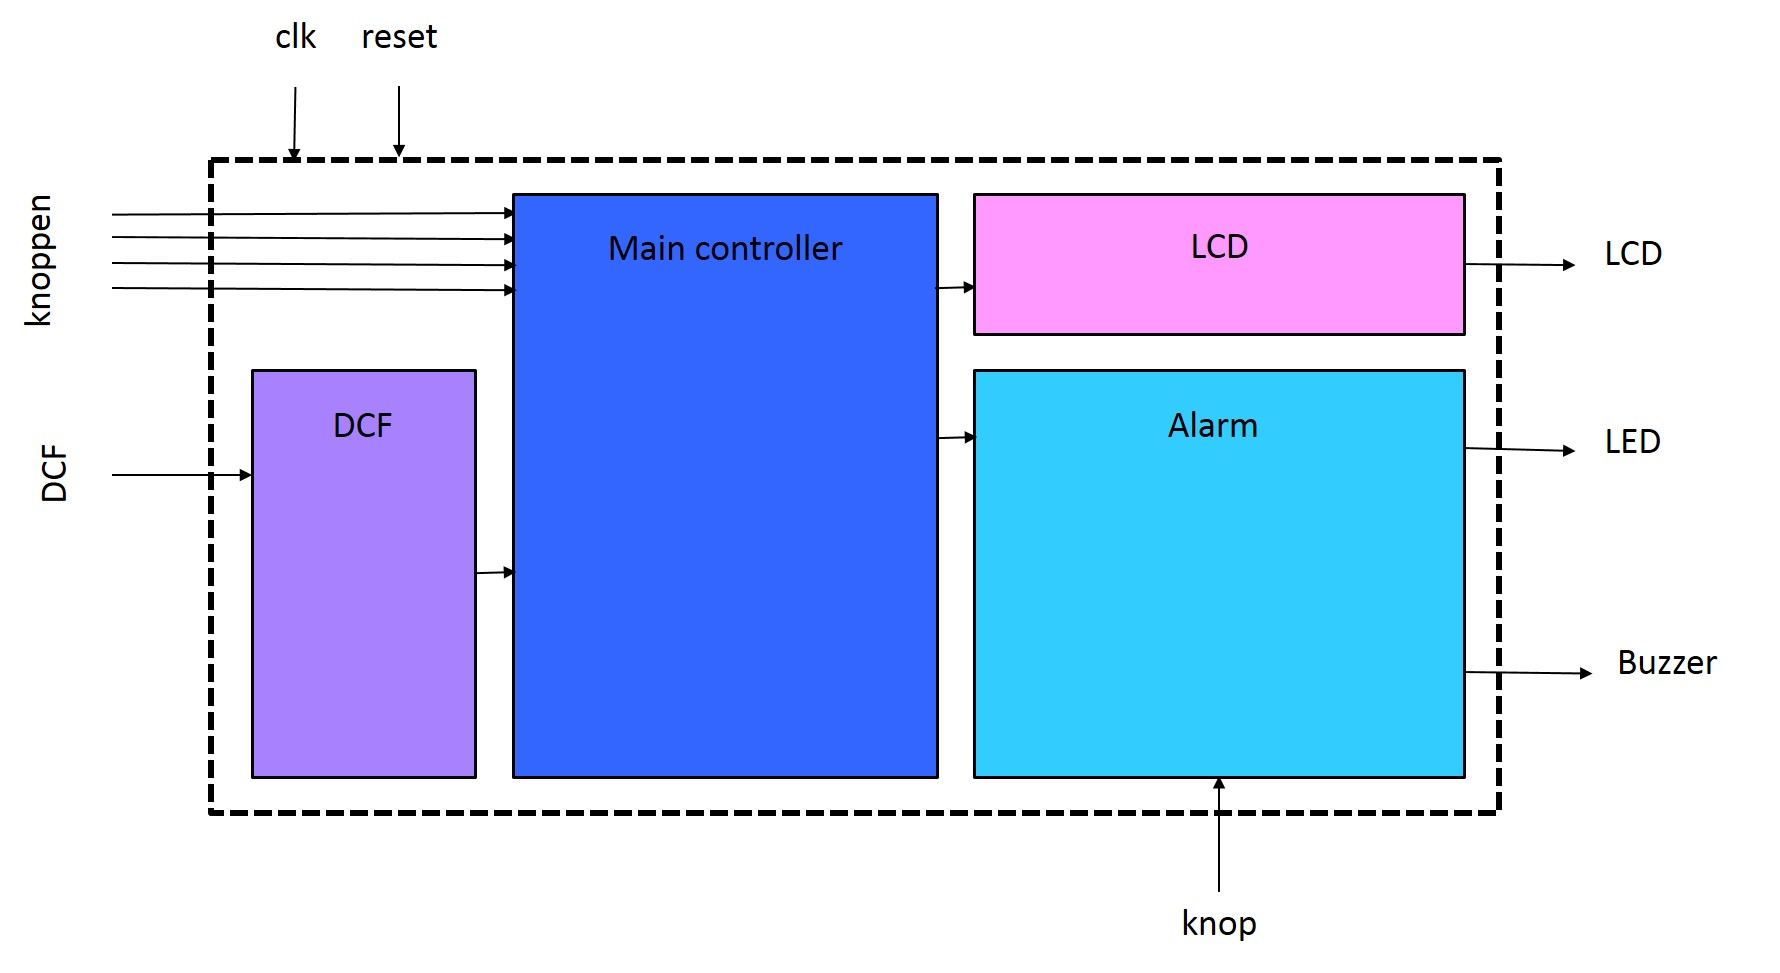
\includegraphics[width=13cm]{figure/blokdiagram}
\caption{Blokdiagram van het gehele systeem}
\label{fig:blokdiagram}
\end{figure}



\end{document}